\documentclass{standalone}
\usepackage{tikz}
\usepackage{ctex,siunitx}
\setCJKmainfont{Noto Serif CJK SC}
\usepackage{tkz-euclide}
\usepackage{amsmath,wasysym}
\usetikzlibrary{patterns, calc,3d}
\usetikzlibrary {decorations.pathmorphing,decorations.pathreplacing,decorations.shapes}
\tikzset{label style/.append style={font=\small}}
\begin{document}
\small
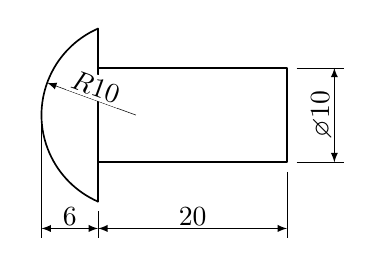
\begin{tikzpicture}[>=latex,scale=1.2,inner sep=1pt]
  \tkzDefPoints{0/0/O,-1/0/R,-0.4/-0.5/A,1.6/-0.5/B,1.6/0.5/C,-0.4/0.5/D}
  \tkzInterLC(A,D)(O,R)\tkzGetPoints{M}{N}
  \tkzDrawArc[semithick,black](O,M)(N)
  \tkzDrawPolygon[semithick](A,B,C,D)
  \tkzDrawSegments[semithick](M,N)
  \draw[very thin,->](O)--++(160:1)node[midway,above,sloped,fill=white]{$R10$};
  \draw[very thin](-1,-0.1)--(-1,-1.3)([yshift=-1mm]N)--++(0,-0.28)(1.6,-0.6)--(1.6,-1.3)(1.7,0.5)--(2.2,0.5)(1.7,-0.5)--(2.2,-0.5);
  \draw[very thin,<->](-0.4,-1.2)--(1.6,-1.2)node[midway,above]{20};
  \draw[very thin,<->](-1,-1.2)--(-0.4,-1.2)node[midway,above]{6};
  \draw[very thin,<->](2.1,-0.5)--(2.1,0.5)node[midway,sloped,above]{$\diameter 10$};
\end{tikzpicture}
\end{document}